\documentclass[11pt,table]{article}

\usepackage{subfiles}
\usepackage[breakable]{tcolorbox}
%\usepackage{parskip} 

\usepackage{iftex}
\ifPDFTeX
\usepackage[T1]{fontenc}
\usepackage{mathpazo}
\else
\usepackage{fontspec}
\fi
\usepackage[english]{babel}
\usepackage{lipsum}
\usepackage{microtype}
\usepackage{float}
\usepackage{caption}


\usepackage{subcaption}
\usepackage[skip=50pt]{caption} % default 10pt
\captionsetup[figure]{skip=10pt}
\usepackage{rotating}
\usepackage{wrapfig}

\usepackage{graphicx}
\graphicspath{
  {figures/}
}  

\captionsetup{format=plain,
	aboveskip=-0.2cm,
	indention=0cm, 
	textformat=simple,
	textfont=small,
	labelfont=small, 
	justification=centering,
	labelfont=bf}



\usepackage[Export]{adjustbox} % Used to constrain images to a maximum size
\adjustboxset{max size={0.9\linewidth}{0.9\paperheight}}
\usepackage{float}
%\floatplacement{figure}{H} % forces figures to be placed at the correct location
\usepackage{xcolor}    % Allow colors to be defined
\usepackage{enumerate} % Needed for markdown enumerations to work
\usepackage{geometry}  % Used to adjust the document margins
\usepackage{amsmath}   % math symbols
\usepackage{amssymb}   % more math symbols
\usepackage{siunitx}   % write numbers and units nicely
% \usepackage{textcomp}  % defines textquotesingle
\usepackage[           % Literaturverwaltung mit BibLaTeX
  style=ieee,
  sorting=none
]{biblatex}                     
\addbibresource{bibliography.bib} % Pfad Literaturverzeichnis
\usepackage[autostyle=true]{csquotes} % Für BibLaTeX notwendig
\usepackage{upquote}   % Upright quotes for verbatim code
\usepackage{eurosym}   % defines \euro
% \usepackage[mathletters]{ucs} % Extended unicode (utf-8) support
\usepackage{fancyvrb}  % verbatim replacement that allows latex
\usepackage{grffile}   % extends the file name processing of package graphics 
% to support a larger range
\makeatletter % fix for grffile with XeLaTeX
\def\Gread@@xetex#1{%
	\IfFileExists{"\Gin@base".bb}%
	{\Gread@eps{\Gin@base.bb}}%
	{\Gread@@xetex@aux#1}%
}
\makeatother

\usepackage{hyperref}
\usepackage[capitalise]{cleveref}
\Crefname{figure}{Fig.}{Figs.}% {<type>}{<singular>}{<plural>}
\usepackage{acro}

% The default LaTeX title has an obnoxious amount of whitespace. By default,
% titling removes some of it. It also provides customization options.
\usepackage{titling}
\usepackage{longtable} 
\usepackage{booktabs}  
\renewcommand{\arraystretch}{1.2} % more space between table rows

\usepackage[inline]{enumitem}
\usepackage[normalem]{ulem}
% normalem makes italics be italics, not underlines
\usepackage{mathrsfs}

\captionsetup[table]{skip=10pt}


% Colors for the hyperref package
\definecolor{urlcolor}{rgb}{0,.145,.698}
\definecolor{linkcolor}{rgb}{0,0,0}%{.71,0.21,0.01}
\definecolor{citecolor}{rgb}{0,0,0}%{.12,.54,.11}


\title{Predicting Renewable Energy Production Using Machine Learning Methods}
\author{Luis Gentner, Leon Sengün, Dilara Yildiz}
\date{\today}



% Prevent overflowing lines due to hard-to-break entities
\sloppy 

\hypersetup{
	breaklinks=true,  % so long urls are correctly broken across lines
	colorlinks=true,
	urlcolor=urlcolor,
	linkcolor=linkcolor,
	citecolor=citecolor,
}
% Slightly bigger margins than the latex defaults

\geometry{verbose,tmargin=1in,bmargin=1in,lmargin=1in,rmargin=1in}

\newcommand{\ket}[1]{\left|{#1}\right\rangle}
\newcommand{\bra}[1]{\left\langle{#1}\right|}
\newcommand{\braket}[2]{\left\langle{#1}\middle|{#2}\right\rangle}



\usepackage{fancyhdr}
\addtolength{\headheight}{1.2cm} % make more space for the header
\pagestyle{fancy} %plain} % use fancy for all pages except chapter start
\fancyhead[L]{\leftmark}
%\lhead{\includegraphics[height=1.3cm]{logo2}} % left logo
\rhead{
\includegraphics[height=0.6cm]{header.png}}   % right logo
%\renewcommand{\headrulewidth}{0pt} % remove rule below header


\title{Project Title}
\author{Luis Gentner, Leon Sengün, Dilara Yildiz}
\date{\today}

\DeclareAcronym{AE}{
short = AE,
long = autoencoder}
\DeclareAcronym{CNN}{
short = CNN,
long = convolutional neural network}
\DeclareAcronym{GRU}{
short = GRU,
long = gated recurrent unit}
\DeclareAcronym{LSTM}{
short = LSTM,
long = long short-term memory}
\DeclareAcronym{PCA}{
short = PCA,
long = principal component analysis}
\DeclareAcronym{RNN}{
short = RNN,
long = recurrent neural network}
\DeclareAcronym{ARRNN}{
short = ARRNN,
long = autoregressive RNN}
\DeclareAcronym{DWD}{
short = DWD,
long = Deutscher Wetterdienst}
\DeclareAcronym{relu}{
short = ReLU,
long = rectified linear unit}

\begin{document}
\begin{titlepage} 
	\centering 
	\rule{\textwidth}{1pt} 
	\vspace{2pt}\vspace{-\baselineskip} 
	\rule{\textwidth}{0.4pt} 
	\vspace{0.1\textheight} 
	
	
	%%% Adjust your project title here
	{\Huge PREDICTING RENEWABLE ENERGY }\\[0.5\baselineskip] 
	{\Huge PRODUCTION USING }\\[0.5\baselineskip]
	%{\Large }\\[0.5\baselineskip] 
	{\Huge MACHINE LEARNING METHODS} 
	
	
	\vspace{0.025\textheight} 
	\rule{0.3\textwidth}{0.4pt} 
	\vspace{0.1\textheight}
	
	%%% Your names, if long, a "\\" in between may help to make things look better
    {\Large \textsc{Luis Gentner, Leon Sengün, Dilara Yildiz}} 
	
	\vfill 
	
	%%% You can include a nice image from your project here
 	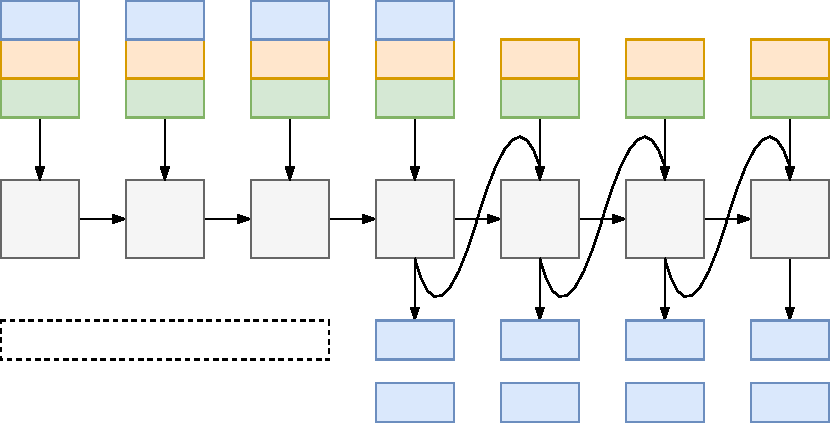
\includegraphics[width=0.5\textwidth]{figures/autoreg-continous-notext.pdf} \\
	\vspace{0.05\textheight}
	{\large\textsc{Machine Learning Methods in Mechanics \\Report}\\ -\\ University of Stuttgart} 
	
	
	\vspace{0.1\textheight} 
	
	%%% Adjust the date here if you like
	{\normalsize \today}
	
	
	\rule{\textwidth}{0.4pt}
	\vspace{2pt}\vspace{-\baselineskip}
	\rule{\textwidth}{1pt}
	
\end{titlepage}

\pagenumbering{roman}
\newpage
\tableofcontents
% ~\\
\printacronyms
\newpage
\pagenumbering{arabic}



\section{Introduction}

The increased share of renewable energies in the total energy mix leads to an increasingly fluctuating power generation. Therefore, measures for a stable energy supply gain importance. Information about future energy production could enable power plant operators to control their plants in advance to match the renewable energy production and customer demand, as well as to avoid paying negative electricity prices. A future prediction could also enable energy storage operators to foresee when energy storage is feasible and when to discharge their storage in a targeted manner. An overview of the German energy mix during one week can be seen in \autoref{fig:Total_Electricity_Wk}.

\begin{figure}[ht]
	\centering
	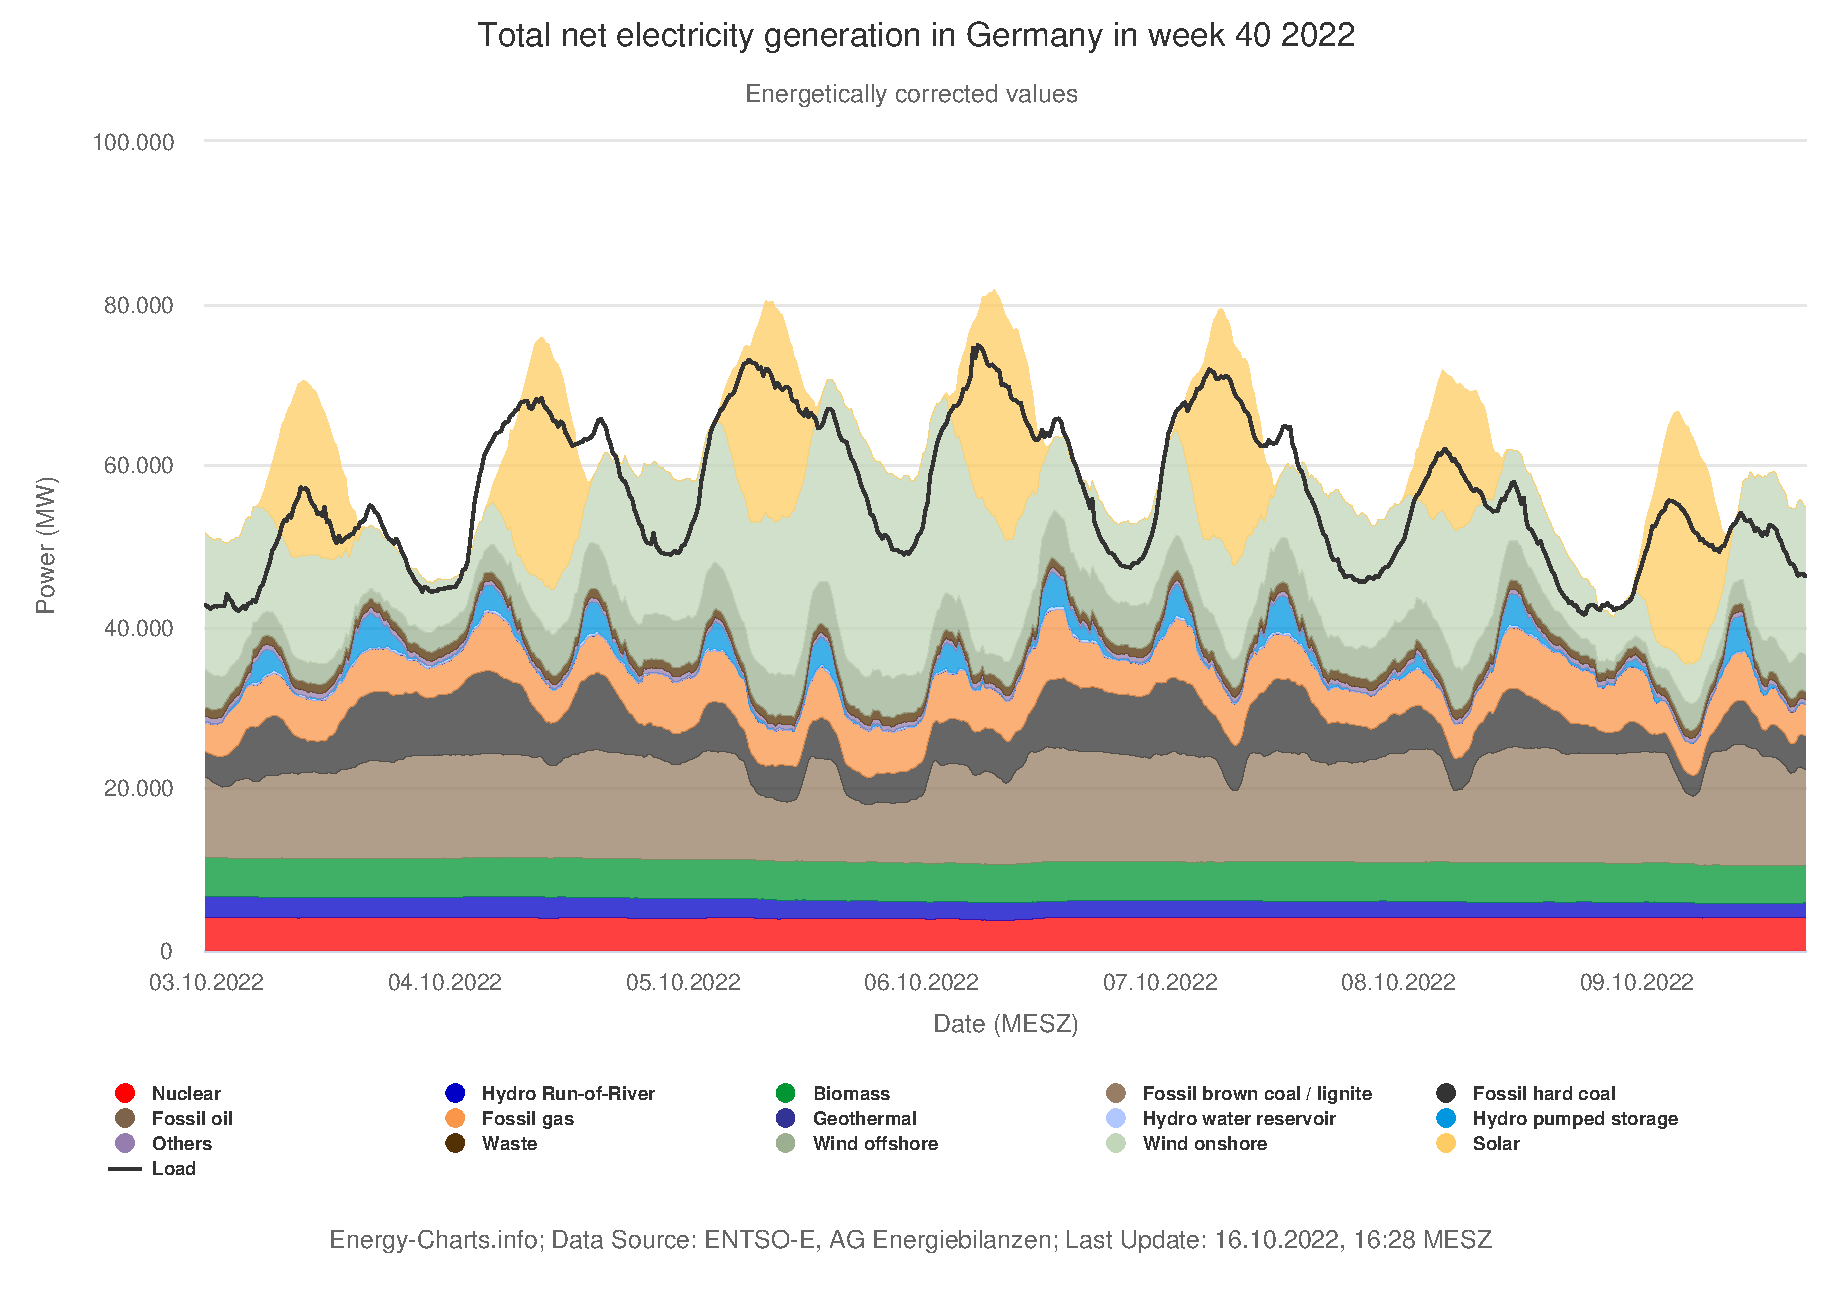
\includegraphics[scale=0.9]{Total_net_electricity_generation_in_Germany}
	\caption{Weekly total net electricity generation in Germany, Week 40, 2022 \cite{energy_charts_stromproduktion}}
	\label{fig:Total_Electricity_Wk}
\end{figure}

With this background, the goal of this work is to develop a machine learning model that predicts the renewable energy production 12 hours into the future.

There are a variety of feasible model architectures to tackle this problem, including \acp{CNN} and \acp{RNN} networks. This paper will first explore and evaluate existing models regarding their accuracy, then iteratively develop an optimized, custom model architecture.

\section{Data acquisition}
\subsection{Data sources}
In order to predict future energy production from renewable sources, data of the energy production in recent years is needed. Old data sets are not representative because the number of solar and wind power plants in operation has increased significantly in recent years \cite{statistaSolarPower, statistaWindPower}. Therefore, years 2017-2021 were selected to train all neural networks in this paper. The solar and wind energy generation highly depends on local weather conditions. To account for this, a second data set of recorded weather parameters from the same time frame was chosen as an optional additional input to the models.
The following data sets were used in this paper:

\begin{itemize}
  \item Electricity data (2017-2021) obtained from Energy-Charts (from Fraunhofer ISE), hourly resolution \cite{energy_charts_stromproduktion}
  \item Weather data (2017-2021) from \ac{DWD} including 117 meteorological stations in Germany, hourly resolution \cite{DWD_API,DWD_Data}
\end{itemize}

\subsection{Feature engineering}
Raw data cannot necessarily be included directly as a feature in the model. Different pre-processing steps and a thoughtful selection of features can significantly improve and are essential for a meaningful prediction.

\begin{figure}[ht]
	\centering
	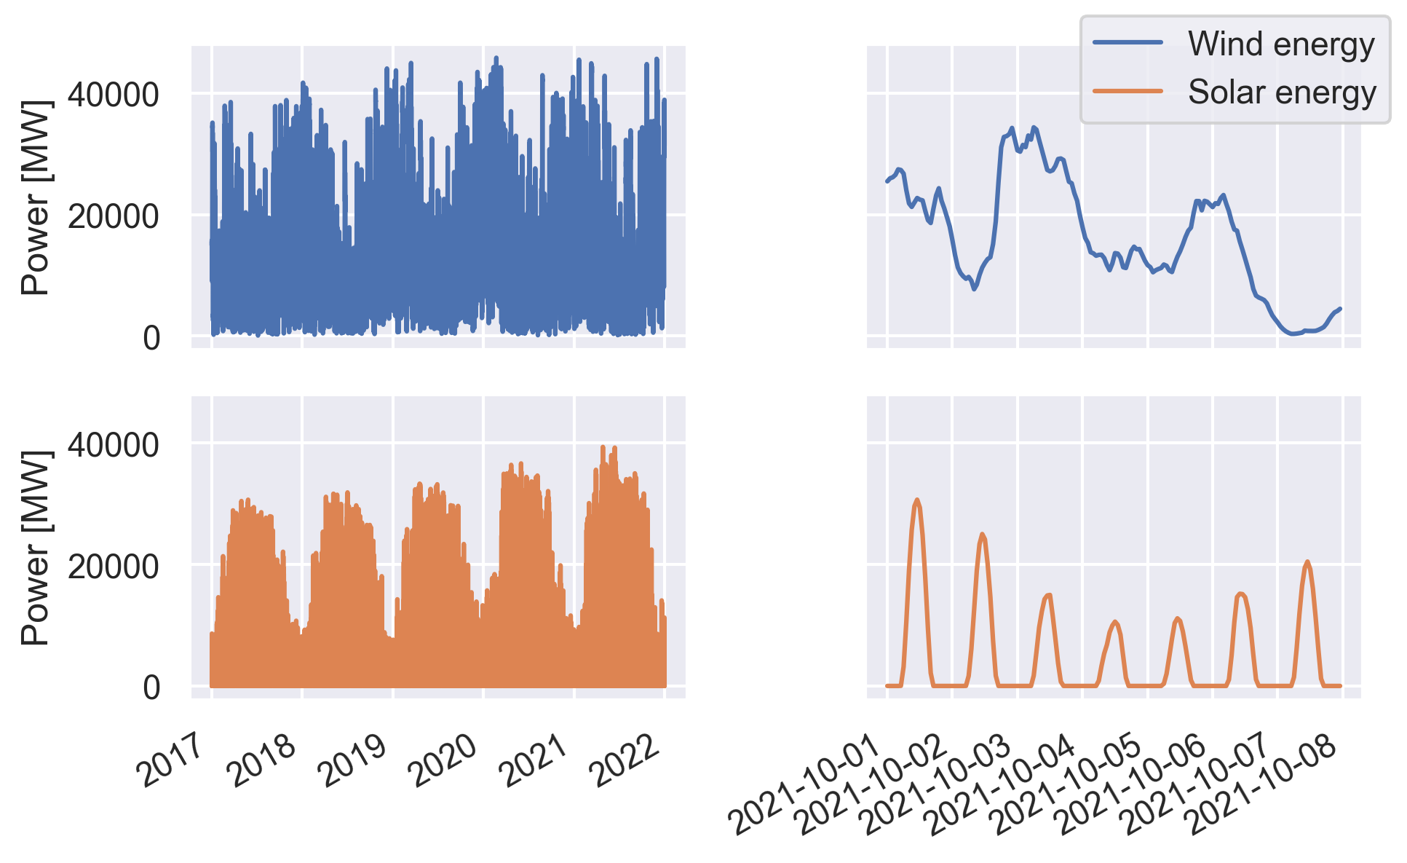
\includegraphics[scale=0.9]{electrData.png}
	\caption{Wind and solar energy production 2017-2021}
	\label{fig:electrData}
\end{figure}

\autoref{fig:electrData} shows the wind and solar energy production of 2017-2021. Seasonal and daily fluctuations can be observed, as well as a year-over-year trend showing a general increase in power. The fluctuations are further investigated with a Fourier analysis, illustrated in \autoref{fig:fourier}.

\begin{figure}[ht]
\centering
\begin{subfigure}{.5\textwidth}
  \centering
  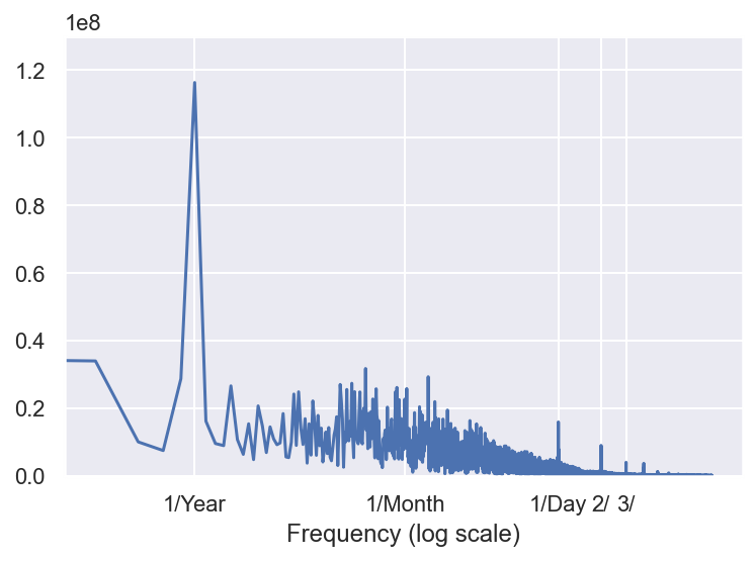
\includegraphics[width=0.9\linewidth]{fourierWind.png}
  \label{fig:fourierWind}
  \caption{Fourier analysis of wind energy production}
\end{subfigure}%
\begin{subfigure}{.5\textwidth}
  \centering
  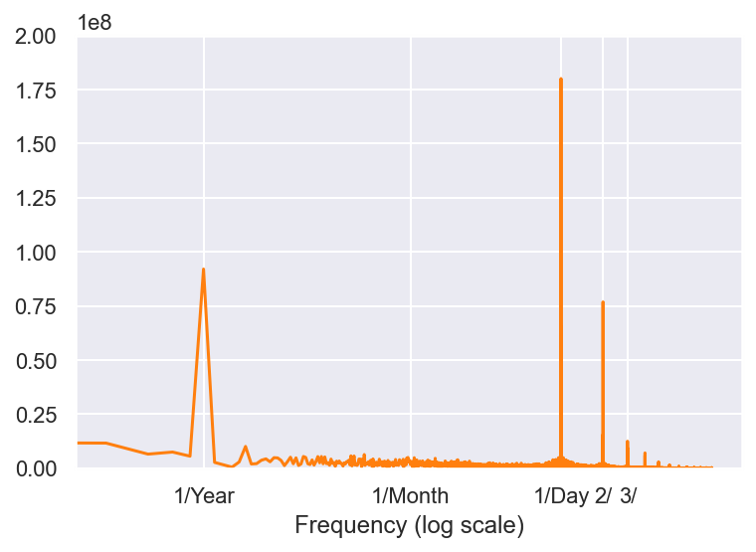
\includegraphics[width=0.9\linewidth]{fourierSolar.png}
  \label{fig:fourierSolar}
  \caption{Fourier analysis of solar energy production}
\end{subfigure}
\caption{Fourier analysis of electricity data}
\label{fig:fourier}
\end{figure}

The Fourier analysis reveals which frequencies appear in the given data. The solar energy production shows the highest peak at a frequency of 1/day, matching the daily elevation of the sun. For both wind and solar energy, the yearly (1/year) and daily (1/day) fluctuations are dominant.
To account for these two frequencies, periodic \textit{time of day} and \textit{time of year} signals were created. Each signal is represented by a sine and a cosine function (\autoref{fig:timeSignal}). 
In addition, two sun elevation features were created. They represent the angle of the sun above or below the horizon, measured at the geometric center of Germany. While the \textit{sun elevation} feature contains positive and negative angles, all negative values of the \textit{clipped sun elevation} feature were set to zero, to account for the almost constant darkness and absence of solar energy production during the night.

\begin{figure}[!htb]
	\centering
	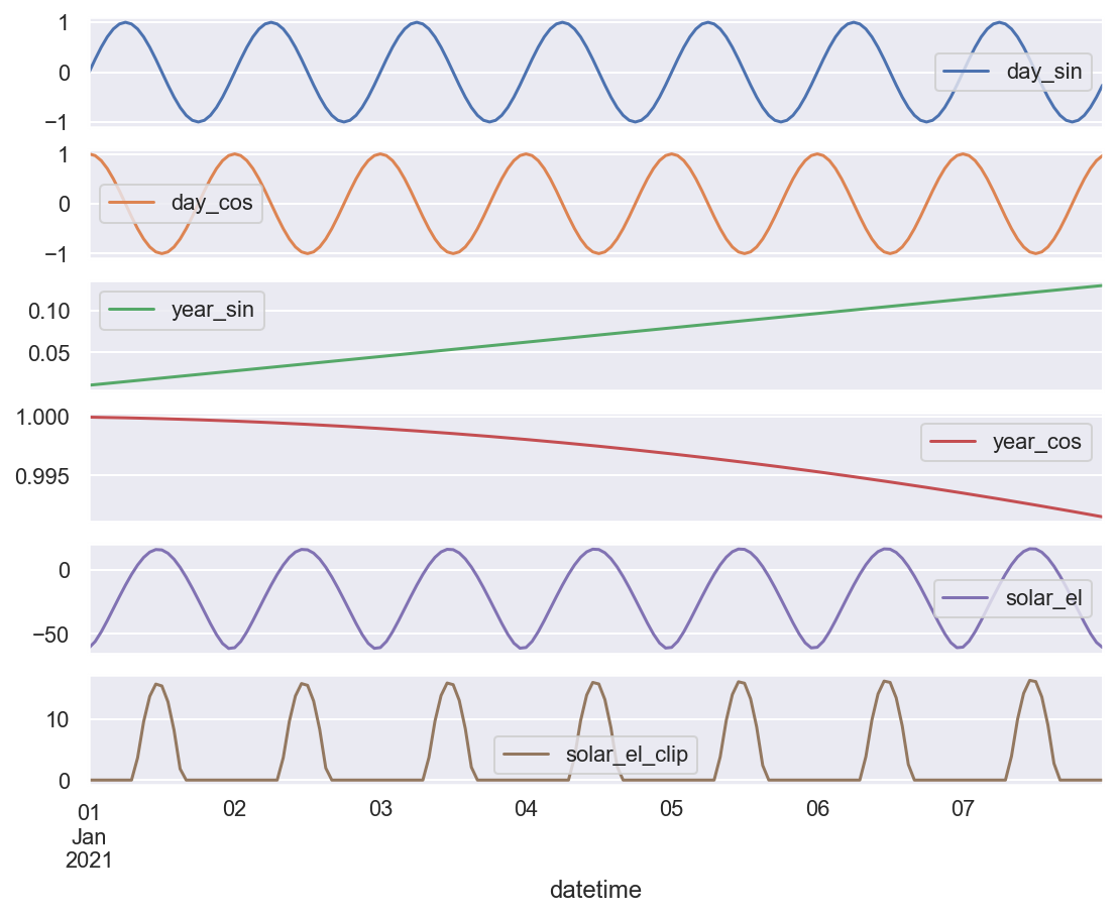
\includegraphics[scale=0.7]{timeSignal.png}
	\caption{Periodic features}
	\label{fig:timeSignal}
\end{figure}

The modified time features as well as air pressure, sunshine duration, temperature and wind speed were subjected to a correlation analysis. 
\begin{figure}[p]
	\centering
	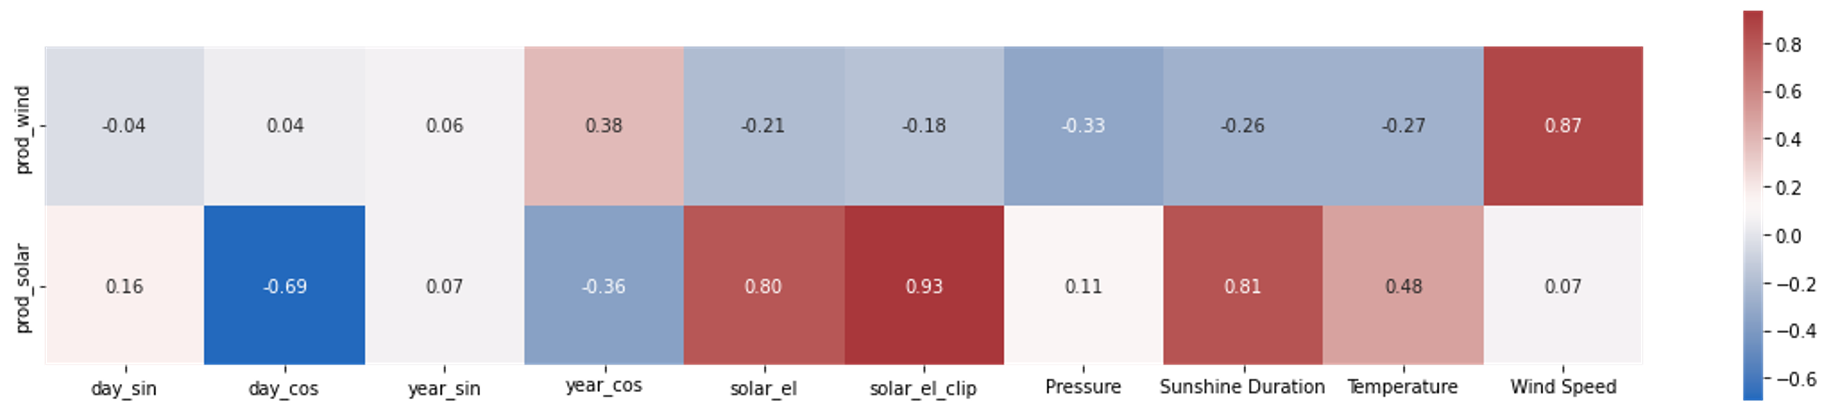
\includegraphics[scale=1]{correlation.png}
	\caption{Correlation analysis}
	\label{fig:correlation}
\end{figure}
\autoref{fig:correlation} shows the correlation matrix. Darker colors indicate a higher (anti-)correlation. The solar energy production is strongly correlated to the cosine of the day, sunshine duration, temperature and clipped solar elevation. As expected, both features correlate strongly with solar energy production, with the \textit{clipped sun elevation} showing the highest correlation (see \autoref{fig:correlation}). In contrast, wind energy production is only strongly correlated to wind speed and the cosine time of year signal. It is slightly correlated to pressure and temperature, because wind energy output is dependent on air density, which is a function of temperature and pressure. Although the sine of day and year do not hold a high correlation, they were included in the feature vector for completeness, since their omission does not significantly reduce the input dimension.
The final feature vector is a combination of 2 energy production features, 6 analytically determined time and solar elevation features, and varying amount of weather features, dependant on the number of selected weather stations. All input features are listed in \autoref{tab:features}.

\begin{table}[p]
    \centering
    \caption{Features}
    \begin{tabular}{lll}
        \toprule
        \textbf{Energy production} & \textbf{Time and solar elevation} & \textbf{Weather} \\ \midrule
        Solar energy prod. & Time of day sine \& cosine     & Temperature*       \\
        Wind energy prod.  & Time of year sine \& cosine    & Wind speed*        \\
                           & Solar elevation                & Pressure*          \\
                           & Clipped solar elevation        & Sunshine duration* \\ \bottomrule
    \end{tabular}
    \\[0.1cm]
    \footnotesize{* Multiple features per weather parameter: One feature per selected \ac{DWD} station}
    \label{tab:features}
\end{table}

\begin{figure}[p]
	\centering
	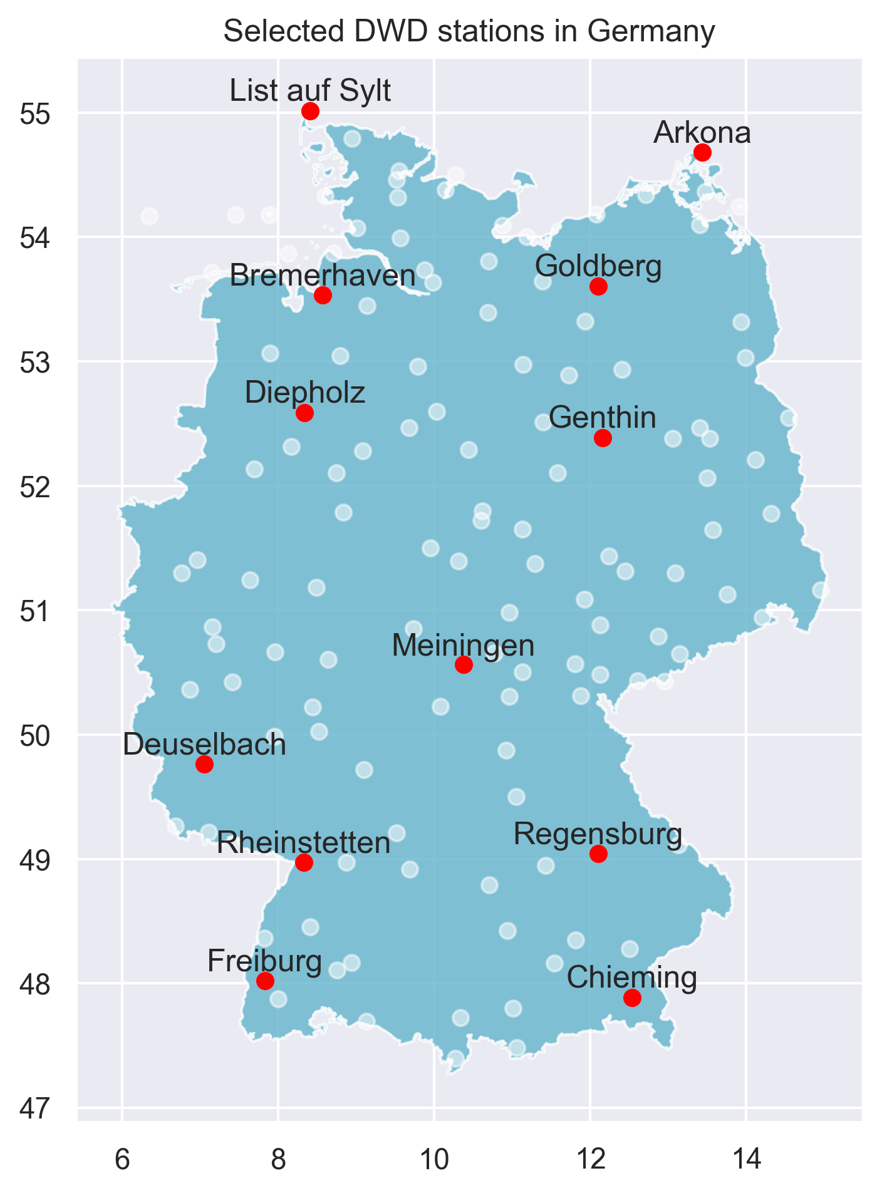
\includegraphics[width=0.5\linewidth]{weatherStations.png}
	\caption{Selected weather stations in Germany. Red points indicate the selected stations, grey points indicate all usable stations that match the required data reliability.}
	\label{fig:weatherStations}
\end{figure}

Out of over 800 meteorological stations in Germany, only 117 provide reliable data for all the required parameters in the time frame of 2017-2021. Of these remaining stations, 12 were selected as an approximate representation of the German weather. Decisive for the selection was the spatial proximity to offshore and solar installations as well as a broad distribution across Germany. The final weather stations are illustrated in \autoref{fig:weatherStations}.

\section{Methods and model architectures} \label{methods}

The goal of this work is to predict solar and wind energy production 12 hours into the future. Current research offers a variety of machine learning models for this problem. Therefore, as a first step, different models were applied to the problem and evaluated regarding their prediction accuracy. Unpromising approaches were then discarded while successful models were further explored and improved. The $R^2$ score was used as a measure of the accuracy of the prediction. The following models were investigated, and were based on the models found in \cite{TF_Timeseries_forecasting}:

\begin{description}
\item[Repeat last step] The non-trainable model repeats the last given time step, leading to a constant solar and wind energy prediction. 
\item[Repeat yesterday] The non-trainable model outputs the time steps with the same local time from the day before. 
\item[Linear] The model consists of one \texttt{Dense} layer with linear activation.
\item[Dense] A deep neural network, consisting of three \ac{relu} activated \texttt{Dense} layers. 
\item[CNN 3x256] Convolutional neural network consisting of one \ac{relu} activated \texttt{Conv1D} layer with 256 filters. The model \textit{CNN 3x256} was fed with the last three time steps.
\item[CNN 24x256] Like the previous model, but this model was fed with the last 24 time steps.
\item[SRNN 32] A \ac{RNN} consisting of one \texttt{SimpleRNN} layer with 32 units. The model is fed with the last 24 time steps and predicts the next 12 time steps in a single shot with an attached \texttt{Dense} layer
\item[GRU 32] Like the previous model, but consisting of a \texttt{GRU} layer. \Acp{GRU} add an update gate in comparison to SimpleRNNs.
\item[LSTM 32] Like the previous model, but consisting of a \texttt{LSTM} layer. \Acp{LSTM} add an forget and output gate in comparison to \acp{GRU}.
\item[LSTM 32$^2$] Deep \ac{LSTM} with two layers each containing 32 units.
\end{description}

Since \acp{RNN} are specialized in time series, a variety of different model architectures were investigates and further developed. 

\subsection{Single-shot \acp{RNN}}
\begin{figure}[hpt]
	\centering
	\input{figures/single-shot.pdf_tex}
	\caption{Single-shot RNN with energy production ($E$) input}
	\label{fig:SRNN}
\end{figure}
Single-shot \acp{RNN} are the simplest recurrent neural networks. After the warmup phase, they predict a predefined number of future steps at once. Although they depict the temporal dependencies in time series, their structure does not allow to vary the length of the prediction output without retraining.

\subsection{\Aclp{ARRNN}}
\begin{figure}[hpt]
	\centering
	\input{figures/autoreg.pdf_tex}
	\caption{\Ac{ARRNN} with energy production ($E$) input}
	\label{fig:ARRNN}
\end{figure}
Autoregressive neural networks work differently: 
The \ac{RNN} cells predict only a single time step into the future. After the warmup phase, the prediction the cell is used as input for the next prediction. This architecture enables a customisable output length without retraining.

\subsection{\Acp{ARRNN} with continuous input}

One disadvantage of the previously described models is that they can not take into account forecasted data that might be available for future time steps. Even though time, solar elevation, and weather forecasts are known for the future, they cannot be included in the previous models due to their given architectures. Therefore, a new model architecture, called \ac{ARRNN} with continuous input, was developed. It makes use of a custom-built Tensorflow model class with modified \texttt{call} and \texttt{warmup} methods. During  \texttt{warmup}, which acts as a \textit{past phase}, the model works like a traditional RNN, where consecutive time steps of power, time, and weather data are fed to an RNN layer. When all available time steps are fed into the layer, it makes a single prediction one time step into the future. During \textit{prediction phase}, the model is only fed with time and weather inputs. In this stage the model works autoregressively - the last power prediction is concatenated with the time and weather inputs and fed into the RNN cell for the next prediction.

\begin{figure}[ht]
	\centering
	\input{figures/autoreg-continous.pdf_tex}
	\caption{\Ac{ARRNN} with energy production ($E$) input and continuous input of time and solar elevation ($T$) and weather parameters ($\textit{WX}$)}
	\label{fig:continousARRNN}
\end{figure}

The continuous \ac{ARRNN} was realized with both \acp{GRU} and \acp{LSTM}. Different numbers of layers and units were investigated.

\subsection{Input compression}
For better predictions, the amount of weather stations could be increased. One possibility would be to directly feed the weather parameters of additional weather stations into the \ac{RNN}. To prevent an overloaded feature vector, the idea was to increase the feature density instead. Therefore, two approaches were tested: Feature compression by using an \ac{AE} and using a \ac{PCA}.

\begin{description}
\item[Autoencoder] An autoencoder was created to verify the quality of the compression. The \ac{AE} inputs and outputs 468 weather parameters of 117 individual \ac{DWD} stations and has a latent space vector of size 48. The latent space representation was then fed into the \ac{RNN}, which means that the number of input features stayed constant to the previous model, that is directly fed with 48 weather parameters of 12 stations. The original, and reconstructed data, as well as the latent space of a single time step are shown in \autoref{fig:AE_Encoding}.
\item[PCA] A linear \ac{PCA} was used to compress the number of features even further, from 468 to 8. The result for a single time step is shown in \autoref{fig:PCA_Encoding}.
\end{description}

\begin{figure}[!htb]
    \centering
    \input{figures/autoenc.pdf_tex}
    \caption{Schematic of the combined \ac{ARRNN} and \ac{AE} model. The energy production ($E$) and time and solar elevation ($T$) input is fed directly into the \ac{ARRNN}, while the weather parameters are first compressed with an \ac{AE} and then fed into the \ac{ARRNN} in their latent space representation.}
    \label{fig:rnn_with_ae}
\end{figure}

\begin{figure}[!htb]
	\centering
	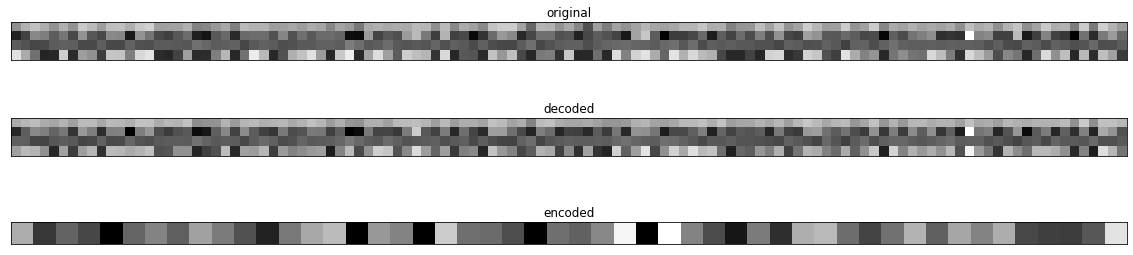
\includegraphics[width=\textwidth]{AE_encoding.png}
	\caption{Original, decoded and encoded weather data using an \ac{AE}}
	\label{fig:AE_Encoding}
\end{figure}

\begin{figure}[!htb]
	\centering
	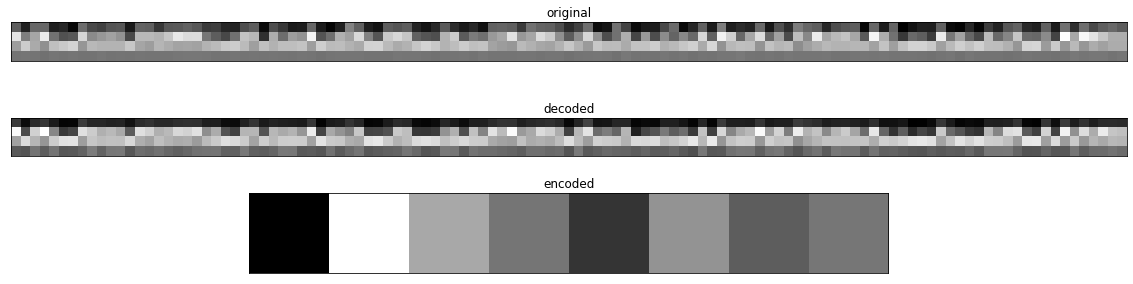
\includegraphics[width=\textwidth]{PCA_encoding.png}
	\caption{Original, decoded and encoded weather data using \ac{PCA}}
	\label{fig:PCA_Encoding}
\end{figure}


\subsection{Final model architecture}

\autoref{fig:modelEvo} shows a summary of the iterative model design process, going from less complex to more advanced models.

\begin{figure}[ht]
	\centering
	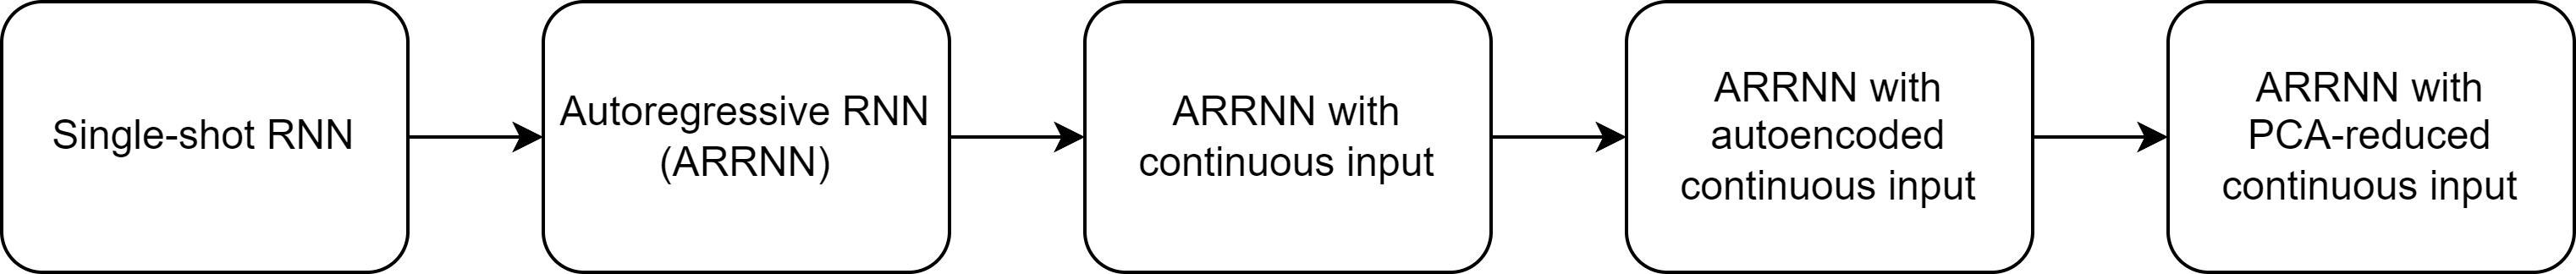
\includegraphics[width=\textwidth]{modelEvolution.png}
	\caption{Iterative model development}
	\label{fig:modelEvo}
\end{figure}

Although the \ac{PCA} can only model linear relationships and compresses the data to only eight features, its performance is almost on par with that of the more complex encoder. Therefore, it was used in the final model:
\begin{itemize}
\item Deep autoregressive \ac{GRU} with continuous input
\item 3 layers [32, 32, 32]
\item Inputs (24 time steps):
\begin{itemize}
\item Solar and wind energy production (during past/warmup phase)
\item 8 time and sun elevation features
\item 8 \ac{PCA} reduced weather features
\end{itemize}
\item Prediction of 12 time steps 
\end{itemize}

\subsection{Optimization}
To further improve the prediction accuracy of the final model, hyperparameter optimization was performed. Due to an incompatible Tensorflow version on the institute server, the optimization was run on desktop-grade hardware. This limited the number of possible optimization trials to 25. Optuna, an open source hyperparameter optimization framework was used to optimize the following three hyperparameters: 
\begin{itemize}
\item Learning rate
\item Units per layer
\item Past input steps
\end{itemize}

\autoref{fig:optimImportance} displays the hyperparameter importances for the trial duration. While learning rate and the number of past steps show a large impact on the duration, the number of units per layer plays only a minor role.

\begin{figure}[ht]
	\centering
	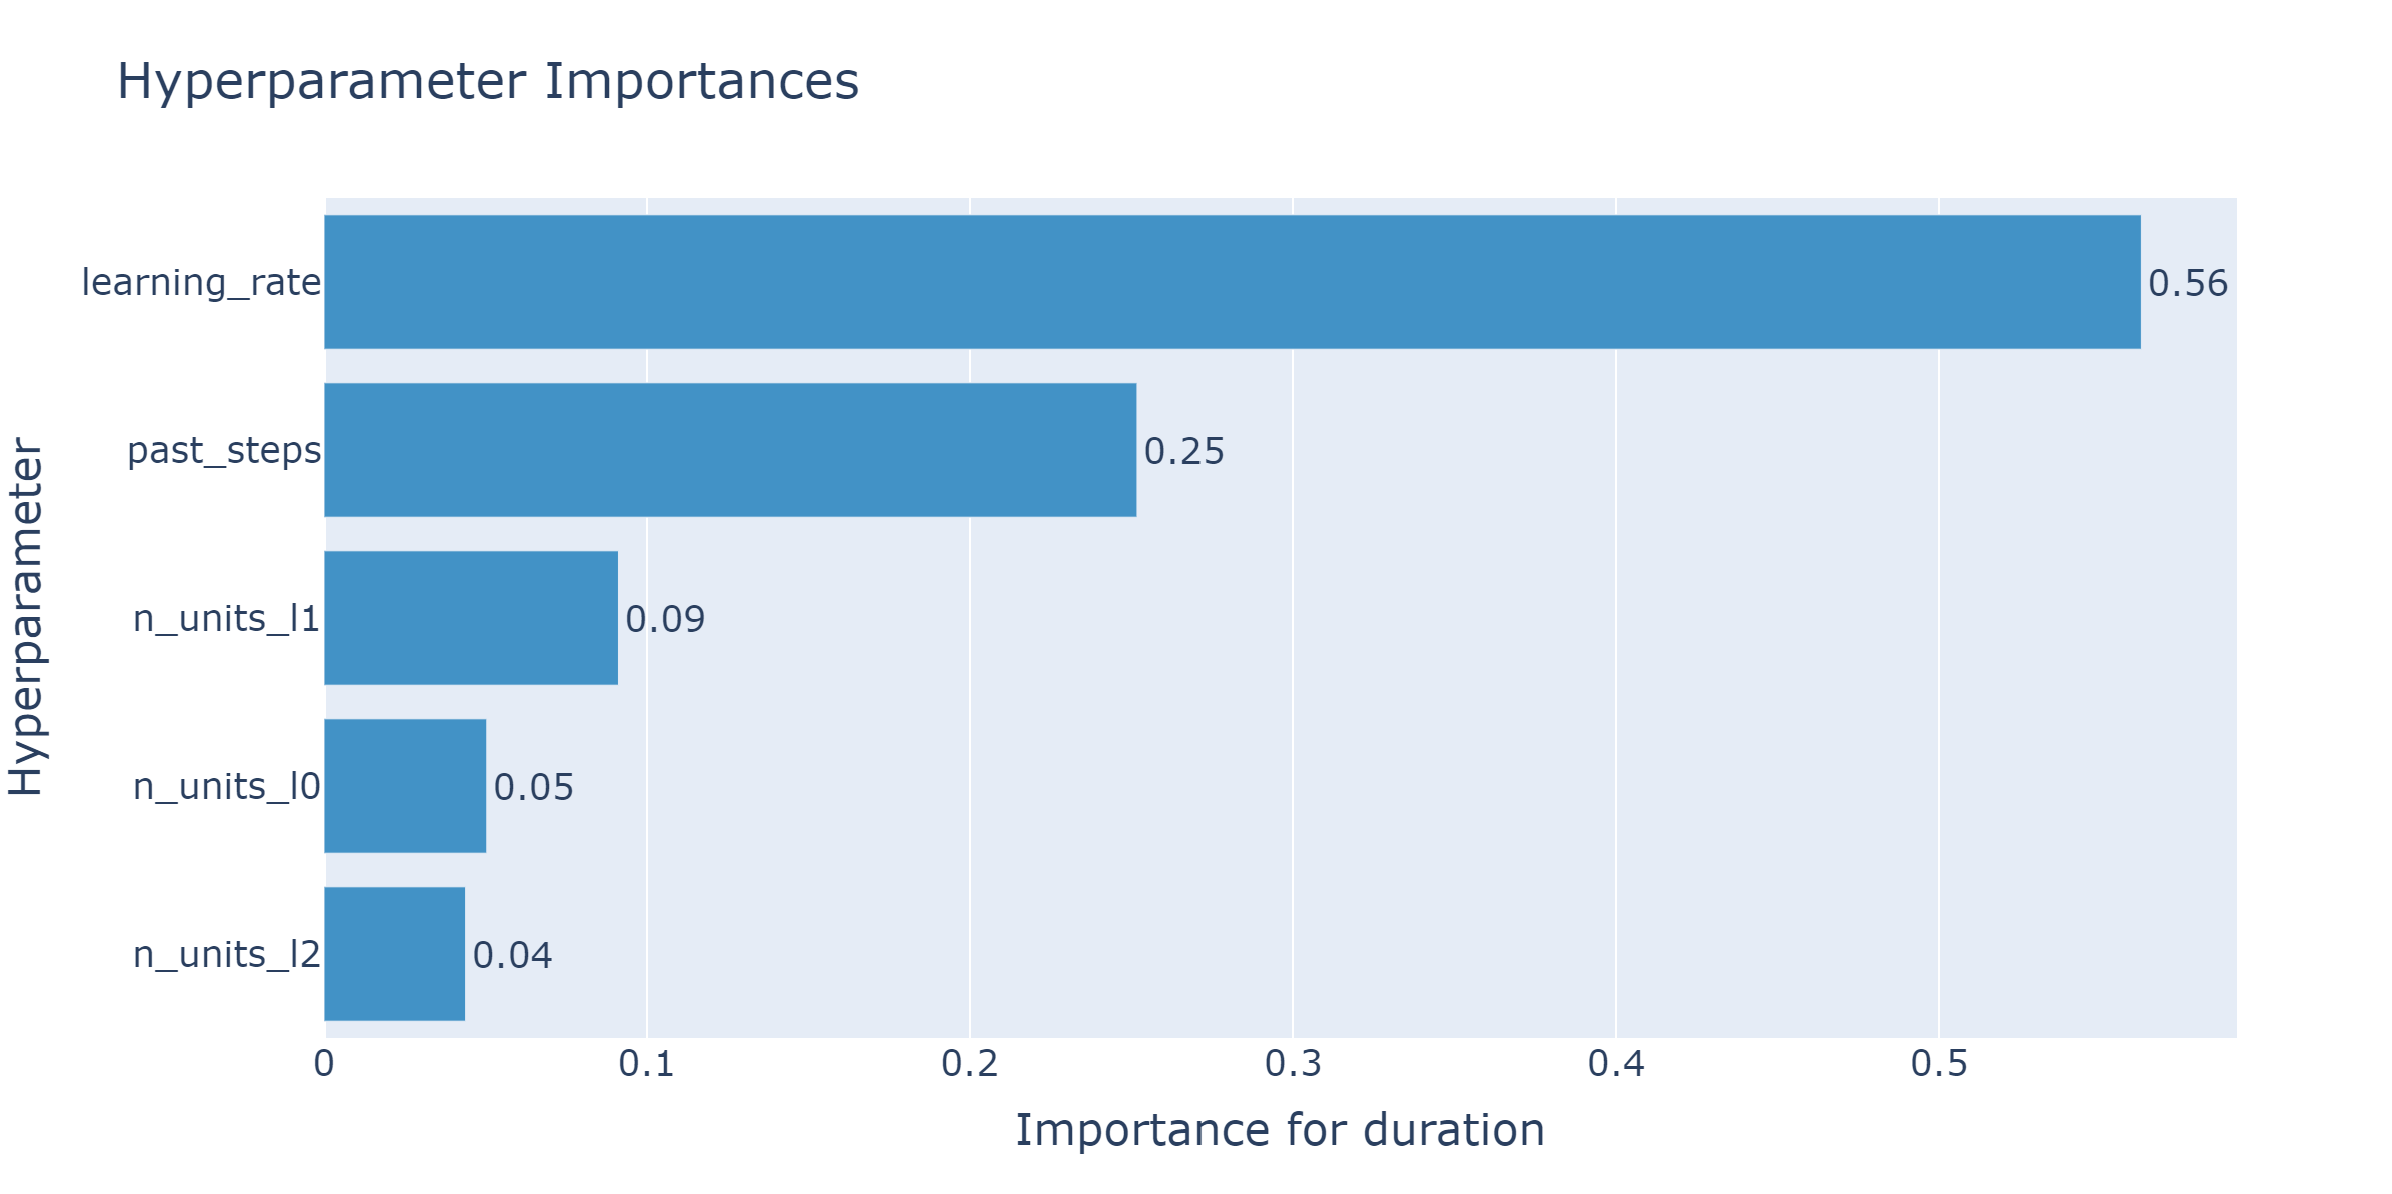
\includegraphics[trim={0 0 0 3cm},clip,width=0.9\linewidth]{optimImportance.png}
	\caption{Hyperparamter importances}
	\label{fig:optimImportance}
\end{figure}

Examining the optimization curve in \autoref{fig:optimHistory}, it can be seen that after the 25 trials, only a minor optimization was achieved, reducing the loss by about $0.005$. In order to further improve the results, optimization should be performed with significantly more trials.

\begin{figure}[ht]
	\centering
	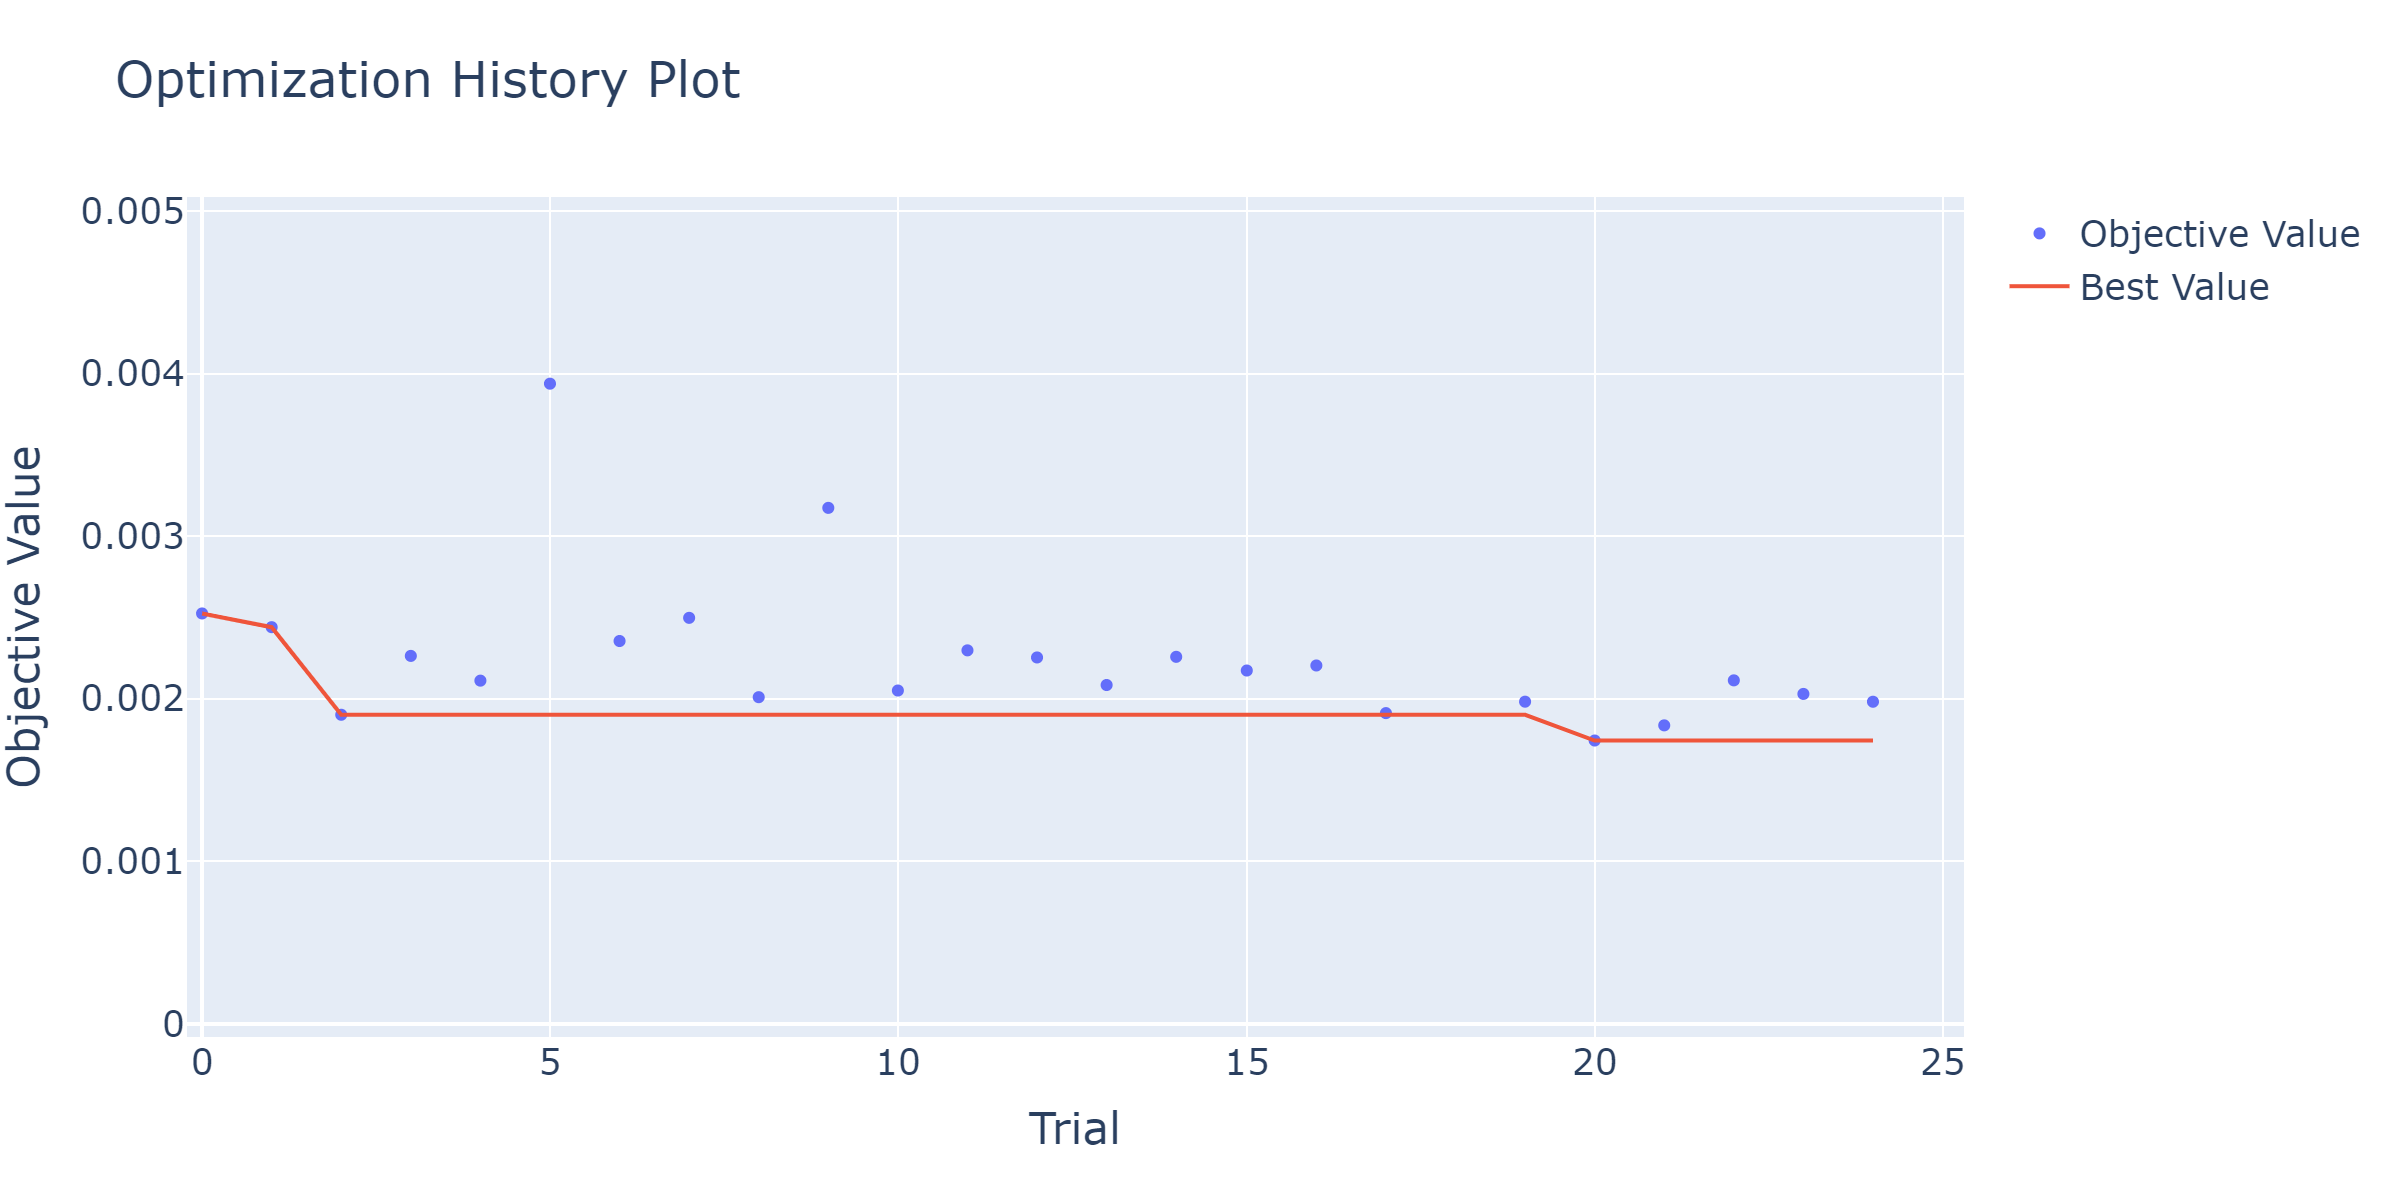
\includegraphics[trim={0 0 0 3cm},clip,width=0.9\linewidth]{optimHistory.png}
	\caption{Hyperparameter optimization history}
	\label{fig:optimHistory}
\end{figure}

\autoref{tab:optimModel} displays the optimized hyperparameters in comparison to the previous model. Striking is a fourfold increase in the number of past steps as well as a higher learning rate. The units per layer were all reduced to 10-15. However, due to the insufficient number of trials, the reliability of the hyperparamter optimization results is questionable. This is also reflected in the $R^2$ score, which differs by only \qty{0.5}{\percent}.

\begin{table}[!htb]
\centering
\caption{Comparison between the non-optimized and optimized final model}
\begin{tabular}{lrr}
\toprule
\textbf{Parameter} & \textbf{Non-optimized model} & \textbf{Optimized model} \\ \midrule
Past steps      & 24         & 92           \\
Learning rate   & \num{5e-4} & \num{1.7e-3} \\
Units 1\textsuperscript{st} layer & 32         & 15            \\
Units 2\textsuperscript{nd} layer & 32         & 10            \\
Units 3\textsuperscript{rd} layer & 32         & 11            \\ \midrule
\textbf{Test} \boldmath$R^2$ \textbf{score}   & \textbf{0.9616}  & \textbf{0.9567} \\ \bottomrule
\end{tabular}
\label{tab:optimModel}
\end{table}

\subsection{Cross-validation}
To ensure that the test and validation data sets were representative for the whole data set and did not skew the model performance, a cross-validation was performed using the K-fold method. For this purpose, the entire data set was split in 5 different subsets, whereby in each fold a different subset served as validation set, while the remaining subsets formed the training set. The model was then trained for each fold separately. The results are listed in \autoref{tab:kfold}. It can be seen that apart from fold 1, the position of the validation set does not have a significant influence on the model performance.

\begin{table}[ht]
\centering
\caption{K-Fold cross-validation}
\begin{tabular}{lrr}
\toprule
\textbf{Fold} & \textbf{Val} \boldmath$R^2$ & \textbf{Test} \boldmath$R^2$ \\ \midrule
1 & 0.9617 & 0.9315  \\
2 & 0.9690 & 0.9574  \\
3 & 0.9686 & 0.9607  \\
4 & 0.9659 & 0.9558  \\
5 & 0.9516 & 0.9444  \\ \midrule
\textbf{Average} & \textbf{0.9633} & \textbf{0.9500} \\ \bottomrule
\end{tabular}
\label{tab:kfold}
\end{table}

\section{Results}
The main idea of this work is to predict the solar and wind energy production 12 hours into the future. Therefore different models and architectures were introduced (\autoref{methods}). In this chapter, the results of these models are presented allowing them to be compared and evaluated. 
%The first part deals with the outcomes of the different models that have been tested. The second discusses the results of the various architectures of \acp{RNN}, particularly the self-developed architecture, the continuous \ac{ARRNN}.

% \begin{figure}[ht]
% 	\centering
% 	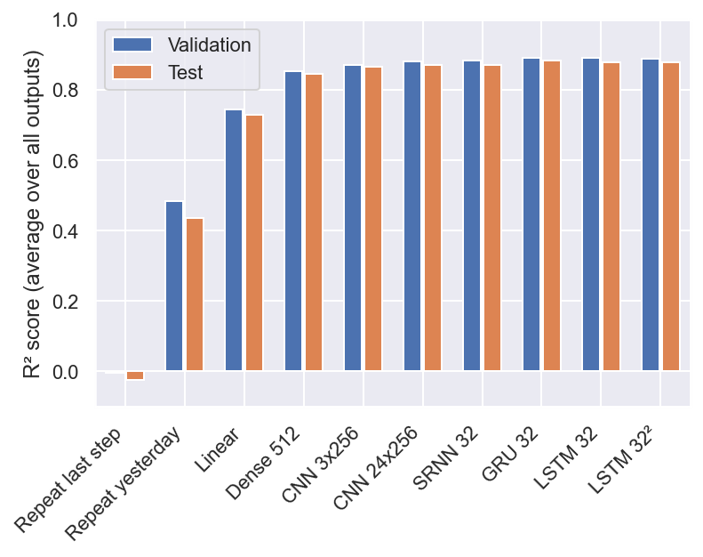
\includegraphics[scale=0.6]{scoresBenchmarks.png}
% 	\caption{$R^2$ scores of benchmark and single-shot prediction networks}
% 	\label{fig:benchmarks}
% \end{figure} 

\autoref{fig:benchmarks} shows the $R^2$ scores, that were reached by the different models. Since the models \textit{Repeat last step} and \textit{Repeat yesterday} only repeat the the energy production input, their performance is very low ($R^2 < 0.5$). While the \textit{Linear} model still shows low accuracy, deep neural network approaches reach scores over 0.8. Recurrent neural networks perform better, because their structure is specialized for time series. The advanced types of recurrent units, \acp{GRU} and \acp{LSTM}, provide the most accurate results and were therefore used for further model development.

As the performance of single-shot \acp{RNN} is limited, more complex network architectures, \acp{ARRNN}, were investigated.

% \begin{figure}[h!]
% \begin{subfigure}{0.5\textwidth}
%     \centering
% 	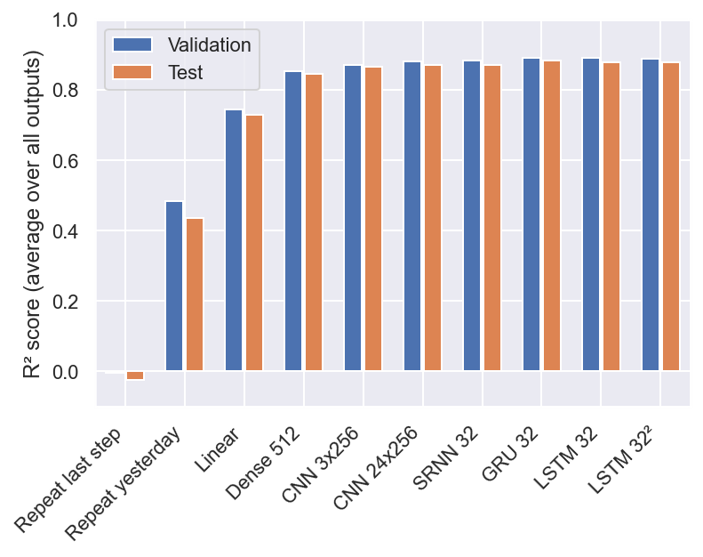
\includegraphics[scale=0.6]{scoresBenchmarks.png}
% 	\caption{$R^2$ scores of benchmark and single-shot prediction networks}
% 	\label{fig:benchmarks}
% \end{subfigure}

% \begin{subfigure}{0.5\textwidth}
% 	\centering
% 	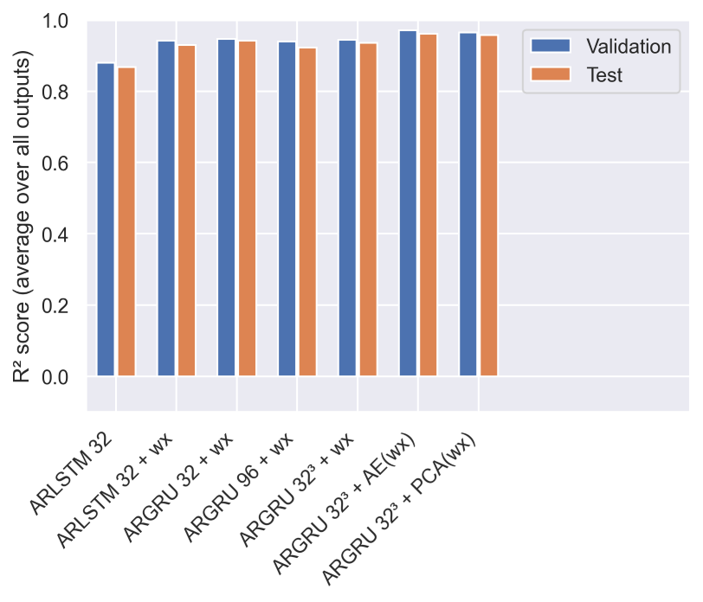
\includegraphics[scale=0.6]{figures/arnnCompare.png}
% 	\caption{$R^2$ scores of different \ac{ARRNN} architectures}
% 	\label{fig:arnnBenchmarks}
% \end{subfigure}
% \end{figure}


\begin{figure}[ht]
\centering
\begin{subfigure}{.5\textwidth}
    \centering
	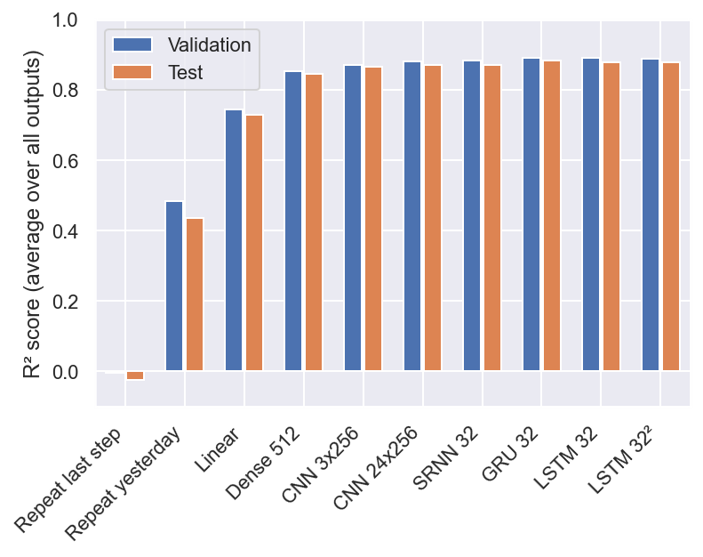
\includegraphics[scale=1.0]{scoresBenchmarks.png} \vspace*{0.5cm}
	\caption{Benchmark and single-shot prediction networks}
	\label{fig:benchmarks}
\end{subfigure}%
\begin{subfigure}{.5\textwidth}
	\centering
	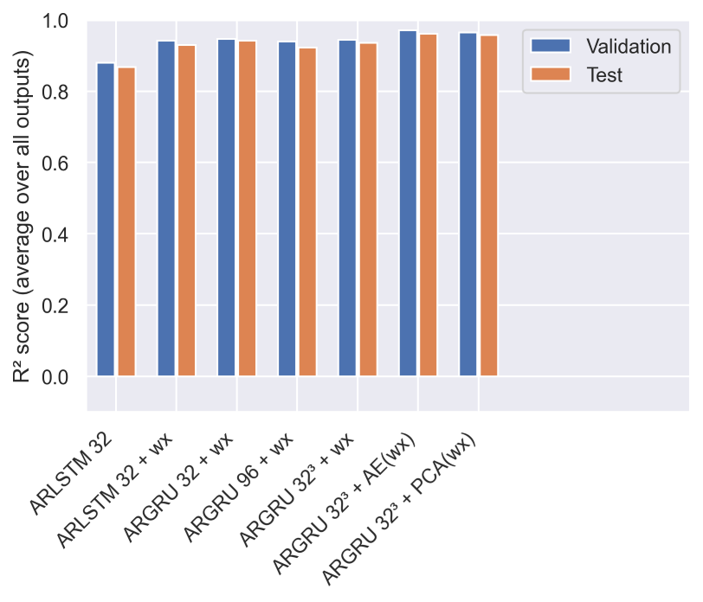
\includegraphics[scale=1.0]{figures/arnnCompare.png}
	\caption{Different \ac{ARRNN} architectures}
	\label{fig:arnnBenchmarks}
\end{subfigure}
\caption{$R^2$ scores of Benchmarks, single-shot prediction networks and \acp{ARRNN}}
\label{fig:ResultBarChart}
\end{figure}



\autoref{fig:arnnBenchmarks} shows the $R^2$ scores of the various autoregressive networks. The number behind the model name indicates the number of layers as well as the number of units per layer. 
\enquote{+ wx} marks the models where weather data was included in form of a continuous \ac{ARRNN}. 
Since \acp{GRU} and \acp{LSTM} were on par regarding their performance, the less complex \acp{GRU} were selected as the basis for advanced model versions with encoder or \ac{PCA}-compressed input.

When the ARLSTM model with 32 units is additionally fed with weather data, a \qty{4}{\percent} increase in the $R^2$ score is achieved. This can be easily explained by the additional, strongly correlating information that is provided, leading to an improved accuracy. The \ac{GRU} shows similar scores to the \ac{LSTM}. However, an increase of the number of units up to 96 resulted in a \qty{2}{\percent} decrease of accuracy. One assumption is that the increased number of trainable parameters cannot be adequately determined due to the limited amount of training data. In contrast, deep \acp{ARRNN}, consisting of three \ac{RNN} layers instead of one, did lead to a slight score improvement.

A further improvement in accuracy was achieved with the encoder and \ac{PCA} reaching $R^2$ scores up to approximately $0.95$. Compressing the weather data including all reliable weather stations in Germany in the encoder or \ac{PCA}, allows the neural network to incorporate more weather information without overloading the feature vector. This compressed weather data input lead to more accurate predictions. However, it is unclear why the ARGRU with upstream \ac{PCA} leads to similarly accurate results than the more complex encoder, despite its linearity and more aggressive compression. One possible explanation is that the important information actually follows linearity and consists of only 8 condensed relevant features. The \ac{ARRNN} with \ac{PCA}-compressed weather data was chosen as the final model, because the reduced input size results in faster training and optimization times.

\begin{figure}[p]
\centering
\begin{subfigure}{\textwidth}
  \centering
  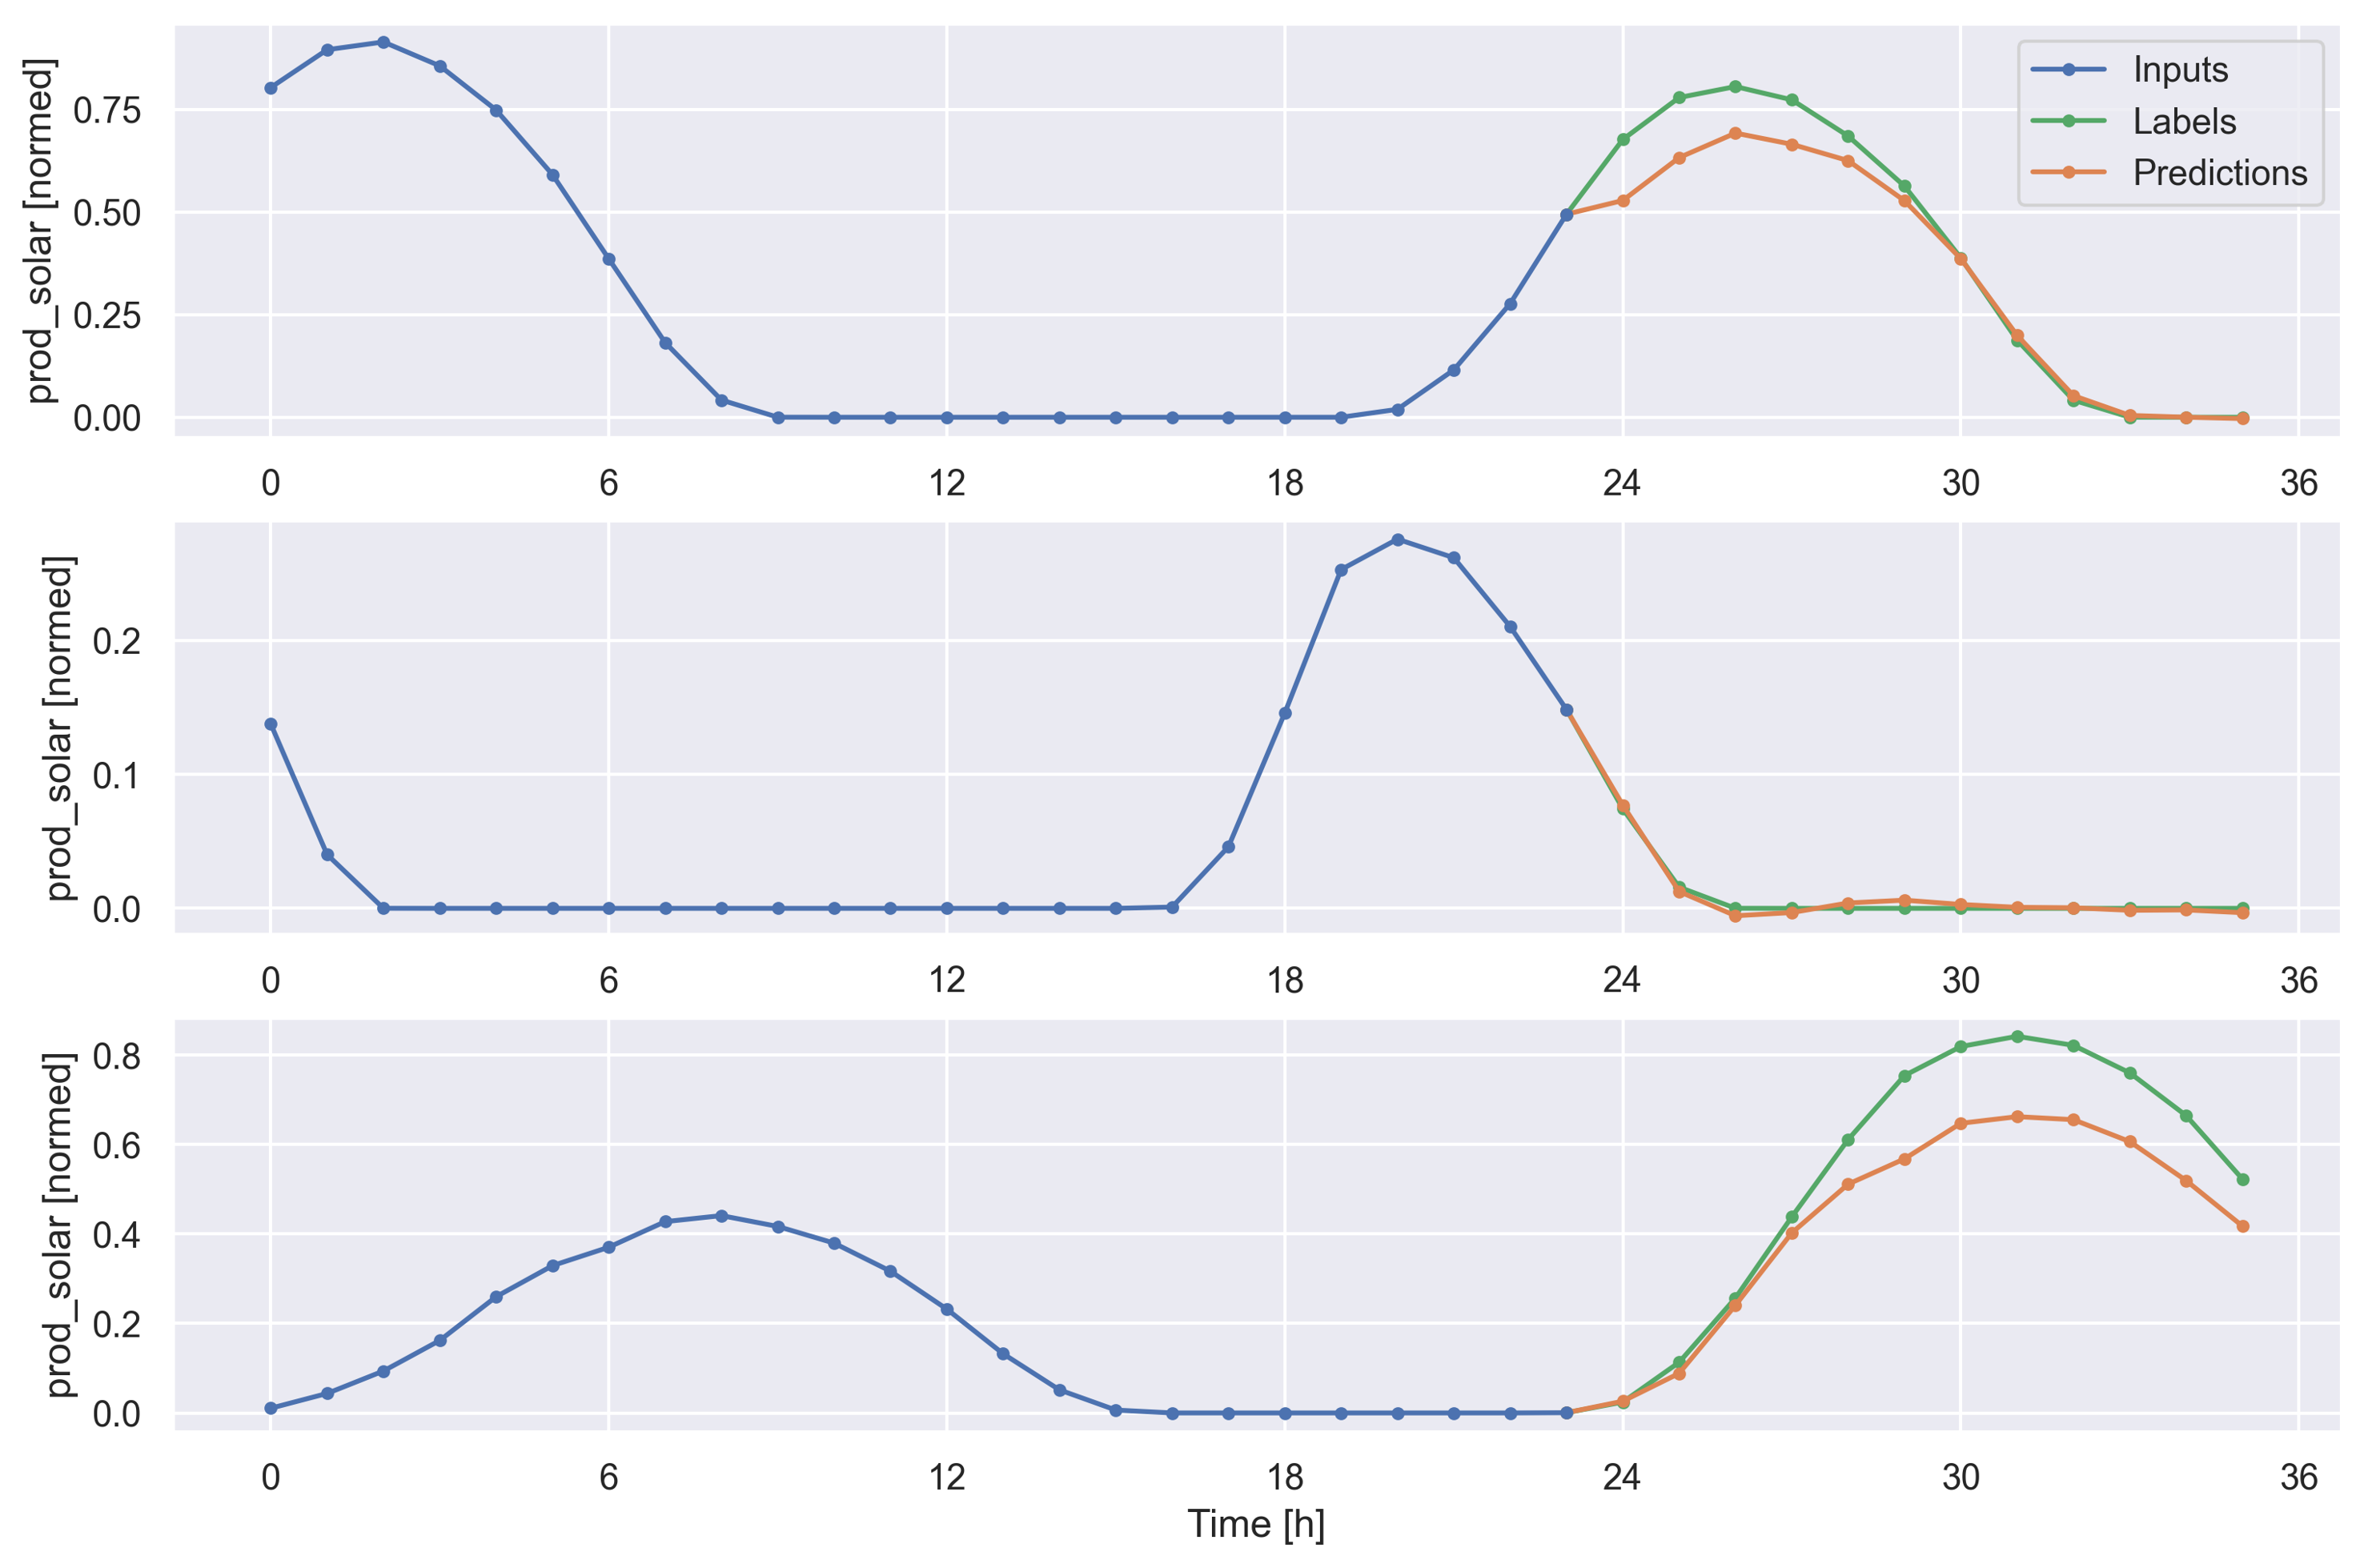
\includegraphics[width=0.8\textwidth]{solarResults.png}
  \label{fig:ResultsWind}
  \caption{Solar energy production}
\end{subfigure}
\begin{subfigure}{\textwidth}
  \centering
  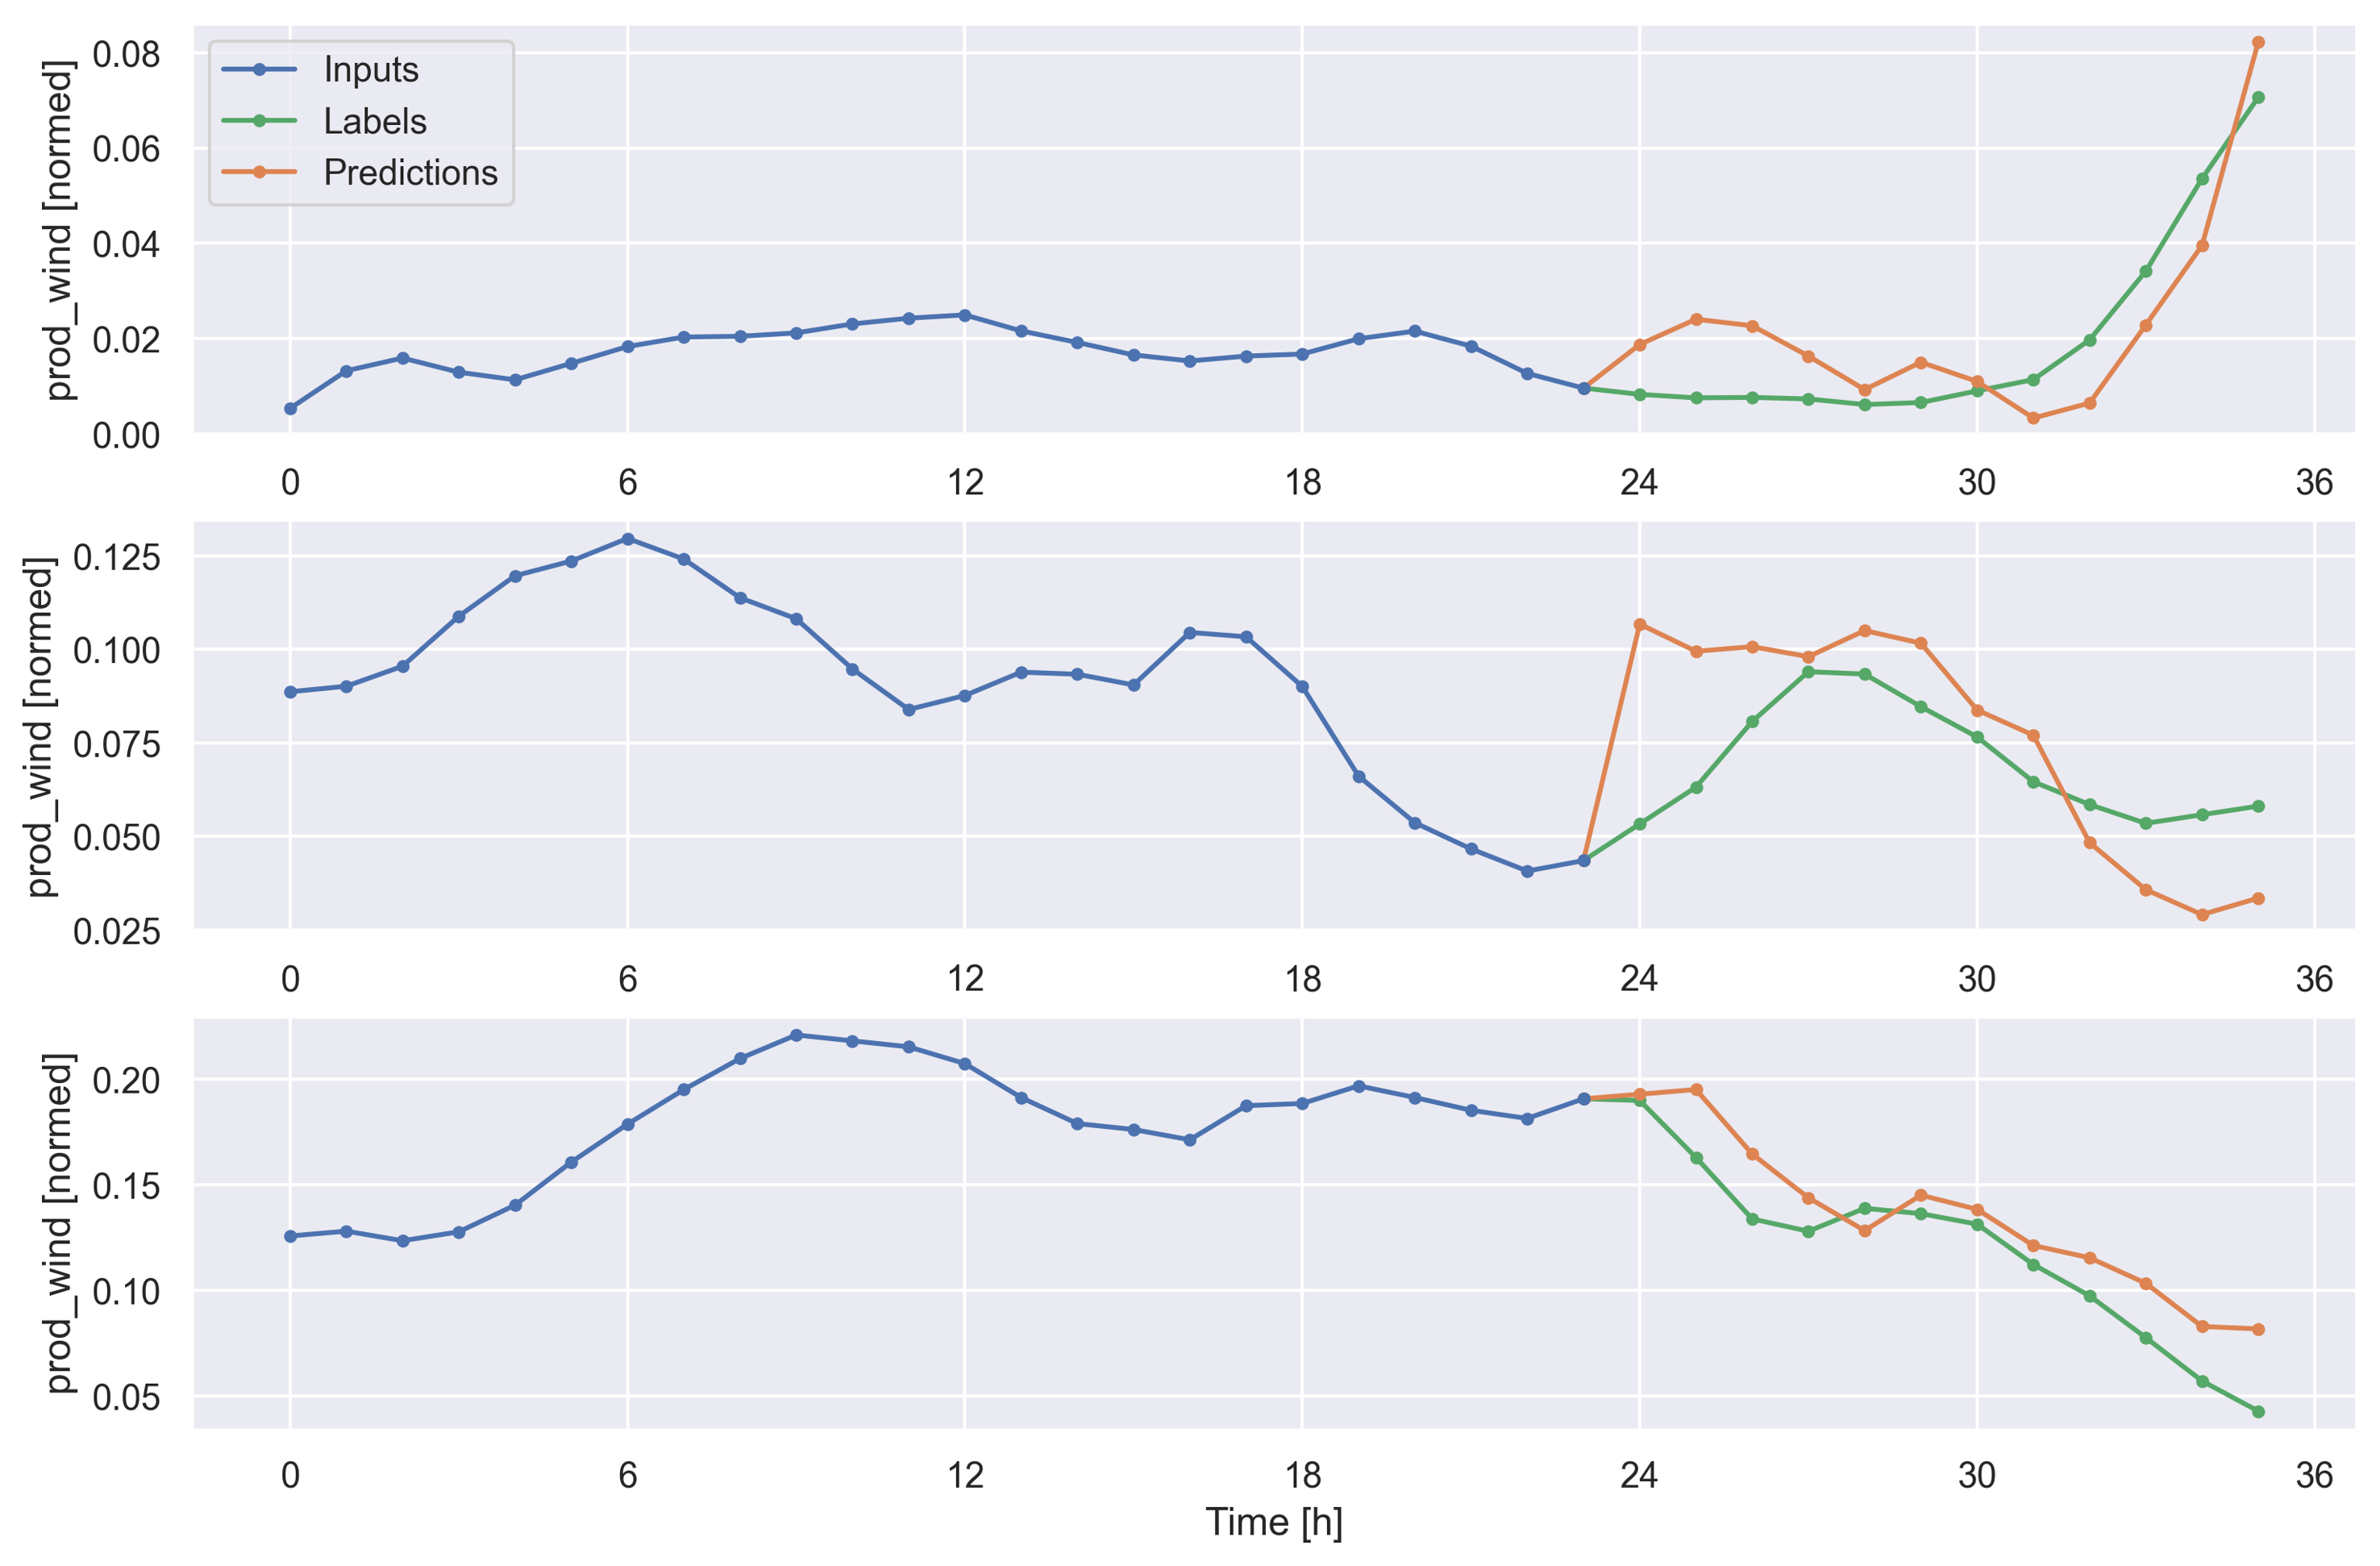
\includegraphics[width=0.8\textwidth]{windResults.png}
  \label{fig:ResultsSolar}
  \caption{Wind energy production}
\end{subfigure}
\caption{Prediction of solar and wind energy production of the final optimized model}
\label{fig:Results}
\end{figure}

\autoref{fig:Results} displays the prediction of solar and wind energy production in randomly selected time frames using the final model. The solar energy predictions are close to the labels with only minor deviations, whereas the wind energy prediction has larger discrepancies from ground truth. The reason can be seen in the correlation analysis (\autoref{fig:correlation}) - while solar energy production is highly correlated with more than three of the given features, wind energy only shows a strong correlation to wind speed. Accordingly, the prediction of wind energy based on these features is also lower.
\newpage
\section{Conclusion}
The goal of this paper was to predict solar and wind energy production 12 hours into the future. Therefore a variety of existing machine learning approaches were investigated and new model architectures were developed. 
%What has been learned from the project is that using \acp{RNN} for this kind of task is favourable because they are best suited for modeling time-series data, and because they offer the ability to be made autoregressive. 
The project has shown that the use of \acp{RNN} is beneficial for these types of tasks, as they are best suited for modeling time series data and also enable autoregressive architectures.
The addition of weather data in the input improved the accuracy of the predictions significantly, especially the prediction of wind power. The particular idea of this work was to also allow future inputs to the autoregressive network to fully exploit available time, sun elevation and weather forecasts for future time steps. For this purpose an autoregressive \ac{RNN} with continuous input was developed, which significantly improved the accuracy of the predictions.
%Furthermore, it became apparent that reducing the dimensionality of the weather data significantly reduces training time and make hyperparameter optimization feasible, without sacrificing accuracy too much.
Furthermore, reducing the dimensionality of the weather data shortened the training time significantly and enabled optimization of the hyperparameters without compromising too much accuracy.
This dimensionality reduction was performed using two methods, an autoencoder and a linear principal component analysis. 
Although \ac{PCA} only maps linear relationships, it achieved similar scores with less complexity and computation time.
A hyperparameter optimization was performed, but due to a lack of processing power, only 25 trials could be completed. Therefore, improvement achieved by the optimization was fairly limited.

\section{Outlook}
Topics that were out of the scope of this project, but could be implemented in a further development include the account for weather forecast inaccuracy by distorting the weather with noise, e.g. a random walk, to account for the increasing uncertainty of the weather forecast over time. Doing a correlation analysis of actual forecast weather data and recorded values for of same time step could reveal the extent of inaccuracy. Testing with real forecast data could reveal the real-world usability of the model in a commercial scenario.

Moreover, by using a \ac{CNN} autoencoder or a graph neural network could help conserve spatial relationships between the weather stations, which are lost by flattening the data set into a vector.

Statistical methods, like Bayesian structural time series \cite{scott_predicting_2014,TFProb_Structural_Timeseries} could be employed as a comparison to the neural network approach.

%% to predict further inputs, such as power consumption, or gas price, which could be used to broaden the scope to include electricity price prediction.
% \newpage
\printbibliography

\end{document}
